% ************************* Preámbulo ********************************

% *************** Document Class ***************
% Para más información sobre las clases:
% https://en.wikibooks.org/wiki/LaTeX/Document_Structure#Document_classes
% En la tabla "Document classes"
% https://ctan.org/topic/class
% \documentclass[10pt, a4paper]{book}
\documentclass[12pt, twoside, a4paper, openright]{book} % \documentclass[options]{class}
% Si usas twoside en vez de oneside, LaTeX te pondrá hojas blancas adicionales

% Para más información sobre las opciones:
% https://en.wikibooks.org/wiki/LaTeX/Document_Structure#Document_classes
% En la tabla "Document Class Options"

% Posibles opciones:
% 10pt, 11pt, 12pt : El tamaño de la fuente por defecto
% a4paper, letterpaper,... : El tamaño del papel del documento
% twocolumn
% landscape
% titlepage, notitlepage
% openright, openany
% draft
% fleqn
% leqno

%------------ Paquetes, macros y metadata ------------%
% ************************ Thesis Information & Meta-data **********************

%------------Información básica------------%
\newcommand{\egilea}{Baldwin David Rodr\'{i}guez Ponce} % The full name of the author
\newcommand{\zuzendariak}{Mar\'{i}a Begoña Losada Pereda}

\newcommand{\upvehu}{Universidad del País Vasco UPV/EHU} % University
\newcommand{\informatikafakultatea}{Facultad de Informática}
\newcommand{\gradua}{Grado en Ingeniería Informática}  % Full title of the Degree
\newcommand{\espezialitatea}{Computación}

\newcommand{\izenburua}{Transpilador de un lenguaje de modelado personalizado de sistemas de simulación dinámicos discretos a
Python} % The title of the thesis
% \newcommand{\izenburua}{Simpy: Un lenguaje de modelado de sistemas de simulación dinámicos discretos} % The title of the thesis
\newcommand{\gapizenburua}{Trabajo de Fin de Grado} % Subtitle
% \newcommand{\gapizenburua}{Proyecto de Fin de Grado}

\newcommand{\crest}{
\includegraphics[width=0.6\textwidth]{1-Portada/FacultadInformatica.jpg}} % University Crest (logo)
\newcommand{\data}{\today} % Submission date
\newcommand{\urtea}{2022}

\newcommand{\egileatestua}{Autor}
\newcommand{\zuzendariaktestua}{Directora}

\newcommand{\abstract}{Resumen}

\message{LaTeX Warning: \noexpand Aviso! Mejor si cambias los textos `Autor/a' y `Directore/a (s)' en funcion del numero y el genero!}

 % Metadata
% ################################################################
% #######     CODIFICACIÓN DEL ARCHIVO              ##############
% ################################################################

% ************************* Input encoding ********************************
% \usepackage{ucs}
\usepackage[utf8]{inputenc} % Permite usar carácteres UTF8
% https://www.overleaf.com/learn/latex/Spanish

% ************************* Output encoding ********************************
\usepackage[T1]{fontenc} % Use 8-bit encoding that has 256 glyphs
% https://www.overleaf.com/learn/latex/Spanish
% \usepackage{courier}

% ************************* Font types ********************************
% times erabili beharrean
\usepackage{mathptmx}
\usepackage[scaled=.90]{helvet}

% ************************* Lenguaje a utilizar ********************************

\usepackage[spanish, es-tabla]{babel} %To extend the default capabilities of LaTeX, providing proper hyphenation and translation of the names of document elements.
% https://www.overleaf.com/learn/latex/Spanish
% \usepackage{hyphenat} % Paquete para controlar la separación de palabras
% \hyphenation{mate-máti-cas recu-perar}



% ################################################################
% #######              GEOMETRY                     ##############
% ################################################################

% ************************* Geometría ********************************
% \usepackage[a4paper, inner=1.5cm, outer=3cm, top=4cm, bottom=3cm, bindingoffset=1cm]{geometry}
% \usepackage[a4paper, left=37mm,right=30mm,top=35mm,bottom=30mm]{geometry}
% \usepackage[left=2.5cm, right=3.5cm, top=4.0cm, bottom=3.0cm]{geometry}
\usepackage[a4paper, inner=2.0cm, outer=3.5cm, top=4.0cm, bottom=3.0cm, marginpar=2.0cm, headheight=14.5pt, showframe]{geometry}

% use option "showframe" in geometry to see frames
% \usepackage[showframe]{geometry}

% ************************* Layout visualization ********************************

\usepackage{layout} % To see the layout of the page
% \usepackage{showframe}


% ################################################################
% #######     ESTILOS EN GENERAL                    ##############
% ################################################################

% *********************** Cabeceras ******************************
\usepackage{fancyhdr} % Permite cambiar el estilo de las cabeceras y pies de página de las páginas del documento
% https://ctan.javinator9889.com/macros/latex/contrib/fancyhdr/fancyhdr.pdf

% \usepackage{fncychap} % Este paquete permite cambiar el estilo de la cabecera de los capítulos
\usepackage[sf,outermarks]{titlesec} % Este paquete permite cambiar el estilo de las cabeceras, pies de página y la forma de las secciones y divisores de sección.
% \usepackage[compact]{titlesec}
% \usepackage{sectsty}


% ************************* ToC and Index ********************************
\usepackage[nottoc]{tocbibind} % Para añadir las listas de figuras y cuadros a la TOC
% \usepackage[acronym,footnote,nonumberlist,toc]{glossaries}
% Erabilera
% http://en.wikibooks.org/wiki/LaTeX/Glossary
% latexmk erabiliz gero, ikusi http://tex.stackexchange.com/questions/1226/how-to-make-latexmk-use-makeglossaries

% Glosario-en eskuliburu zabaldua
% http://osl.ugr.es/CTAN/macros/latex/contrib/glossaries/glossaries-user.html#x1-140002.2
\usepackage[page]{appendix} % Añade el enviroment appendices
% \usepackage[toc,page]{appendix} % Añade una tabla de apéndices a la ToC
% https://osl.ugr.es/CTAN/macros/latex/contrib/appendix/appendix.pdf
% \addto{\captionsspanish}{
%     \renewcommand*{\appendixpagename}{Ap\'{e}ndices}
%     \renewcommand*{\appendixtocname}{Ap\'{e}ndices}
% }
\usepackage{makeidx} % Para crear el index si existe

% *********************** Global paragraph indentation ******************************
\usepackage{parskip} % El único propósito es quitar el indent de todos los párrafos
\usepackage{setspace} % spacing environment
%\usepackage[protrusion=true,expansion=true]{microtype}



% ################################################################
% #######     COLOURS                               ##############
% ################################################################

% *************************** Colours *****************************

\usepackage{color}
\usepackage[table, svgnames, pdftex,dvipsnames]{xcolor} %  Coloured text etc.
% https://ctan.javinator9889.com/macros/latex/contrib/xcolor/xcolor.pdf
\usepackage{colortbl}



% ################################################################
% #######     GRAPHICS                              ##############
% ################################################################

% *************************** Graphics and figures *****************************
\usepackage{epsf, graphics, graphicx}

\usepackage[figuresright]{rotating}
%\usepackage{wrapfig}

\usepackage{float} % Fuerza las figuras a una posición exacta

\usepackage[font=small,labelfont=bf]{caption}
\usepackage{subcaption} % Permite poner subsubtítulos dentro de figuras compuestas
% http://mirrors.ibiblio.org/CTAN/macros/latex/contrib/caption/subcaption.pdf

% \usepackage{tikz} % Advanced inline graphics.
% % https://www.bu.edu/math/files/2013/08/tikzpgfmanual.pdf
% % https://ctan.javinator9889.com/graphics/pgf/base/doc/pgfmanual.pdf
% \usepackage{pgfplots}
% \usetikzlibrary{shapes, decorations, calc, arrows}
% \usetikzlibrary{3d,fit,backgrounds, decorations.text}
% \usetikzlibrary{positioning, shapes.symbols}
% \usetikzlibrary{decorations.pathreplacing, calligraphy}
% \tikzset{>=latex}



% ################################################################
% #######     MATHEMATICS                           ##############
% ################################################################

% ************************* Mathematics ********************************
\usepackage{amsmath}
\usepackage{amssymb}
% \usepackage{amsthm} % Use ntheorem better
\usepackage{ntheorem} % Customizing and writing theorems
\usepackage{bm} % Bold math symbols
\usepackage{amscd}
\usepackage{latexsym} % Even more operators. http://mirrors.ibiblio.org/CTAN/macros/latex/base/latexsym.pdf
\usepackage{calc} % Para hacer cálculos de longitudes en los comandos

% *********************************** SI Units *********************************
\usepackage{siunitx} % use this package module for SI units


% ************************* Text typesetting extras ********************************
\usepackage{csquotes} % Para permitir citas en el texto (bonitas)
\usepackage{circledsteps} % Permite crear texto y números encerrados en círculos
% \usepackage[activate=true, final, tracking=true, kerning=true, spacing=true, factor=1100, stretch=10, shrink=10]{microtype}
% \usepackage{microtype}

\usepackage{lipsum}                     % Dummytext
\usepackage{xargs}                      % Use more than one optional parameter in a new commands

% ################################################################
% #######     INSERTABLES                           ##############
% ################################################################

% ************************* Beatiful colorboxes (breakable) ********************************
% \usepackage{mdframed}
\usepackage[most]{tcolorbox} % https://osl.ugr.es/CTAN/macros/latex/contrib/tcolorbox/tcolorbox.pdf

% ******************************* Itemize and enumerate *********************************

\usepackage{paralist} % compactenum...
\usepackage{enumitem} % Customizable enums
% https://ctan.javinator9889.com/macros/latex/contrib/enumitem/enumitem.pdf

% ******************************* Tables *********************************

% https://ctan.javinator9889.com/macros/latex/contrib/booktabs/booktabs.pdf
\usepackage{array} % For defining special column types
\usepackage{ragged2e} % For new types of columns
\usepackage{longtable} % For breakable tables
\usepackage{multirow} % Table cells that span multiple rows
\usepackage{multicol} % Table cells that span multiple columns
% https://osl.ugr.es/CTAN/macros/latex/required/tools/array.pdf
\usepackage{tabulary}
% https://osl.ugr.es/CTAN/macros/latex/contrib/tabulary/tabulary.pdf
\usepackage{xltabular}
% https://www.ctan.org/pkg/xltabular
\usepackage{tabularx}
% https://ctan.org/pkg/tabularx?lang=en
\usepackage{booktabs} % For professional looking tables

% *************************** Listings *****************************

% http://tug.ctan.org/tex-archive/macros/latex/contrib/caption/caption-eng.pdf
% \usepackage{listingsutf8} % - Para escribir código
\usepackage{listings}
% https://www.overleaf.com/learn/latex/Code_listing
% https://osl.ugr.es/CTAN/macros/latex/contrib/listings/listings.pdf

% \usepackage{minted} % Substitute for listings
% https://github.com/gpoore/minted/blob/master/source/minted.pdf
% \usepackage{textcomp} % XML kodea formateatzeko

% *************************** Markdown listings *****************************
\usepackage[smartEllipses]{markdown}

% ************************* Margin Notes ********************************
\usepackage{marginnote}
\usepackage{marginfix}
% \usepackage{mparhack}

% *********************************** TODO Comments *********************************
% \setlength {\marginparwidth }{2cm}
\usepackage[colorinlistoftodos,prependcaption,textsize=scriptsize,textwidth=2cm]{todonotes}


% ################################################################
% #######     REFERENCES AND BIBLIOGRAPHY           ##############
% ################################################################

% ************************* Bibliography ********************************
\usepackage[backend=biber,style=apa,autocite=plain,sorting=ynt]{biblatex}

% ************************* Referencias y enlaces ********************************
\usepackage{url} % https://osl.ugr.es/CTAN/macros/latex/contrib/url/url.pdf

\usepackage[hyperindex,bookmarks,colorlinks=true,citecolor=blue,urlcolor=blue,linkcolor=blue,pdftex,unicode]{hyperref} % Se recomienda que sea el último paquete en ser importado

\usepackage{cleveref} % Clever references (éste debe ser en realidad el último paquete importado)

% line in order to check if utf-8 is properly configured: áéíóúñ
% ################################################################
% #######     CODIFICACIÓN DEL ARCHIVO              ##############
% ################################################################

% ************************* Input encoding ********************************

% ************************* Output encoding ********************************
\DeclareSymbolFont{usualmathcal}{OMS}{cmsy}{m}{n}
\DeclareSymbolFontAlphabet{\mathcal}{usualmathcal}

% ************************* Lenguaje a utilizar ********************************
\addto\captionsspanish{
	\renewcommand{\contentsname}{Tabla de contenidos}
	\renewcommand{\listtablename}{\'{I}ndice de tablas}
	\renewcommand{\listfigurename}{\'{I}ndice de figuras}
	\renewcommand{\lstlistlistingname}{\'{I}ndice de códigos}
	\renewcommand{\tablename}{Tabla}
	\renewcommand{\appendixname}{Anexo}
	\renewcommand{\appendixpagename}{Anexos}
	\renewcommand{\appendixtocname}{Anexos}
	\renewcommand{\lstlistingname}{Código} % Listing -> Listado
}
% ################################################################
% #######              GEOMETRY                     ##############
% ################################################################

% ************************* Geometría ********************************
% ################################################################
% #######     ESTILOS EN GENERAL                    ##############
% ################################################################

% *********************** Cabeceras ******************************

% ************ Headers, Footnotes and others ************
\setlength{\headheight}{15.13202pt} %not working?

% % De las cabeceras y pies de página de cada página:
\fancypagestyle{empty}{ %
    \fancyhf{} % remove everything
    \renewcommand{\headrulewidth}{0pt} % remove lines as well
    \renewcommand{\footrulewidth}{0pt}
}

% Redefine plain page style
\fancypagestyle{plain}{
	\fancyhf{}
	\renewcommand{\headrulewidth}{0pt}
	\fancyfoot[LE,RO]{\thepage}
}

\fancypagestyle{fancy-intro}{%
    \fancyhf{}
    \fancyhead[RE]{\textit{\nouppercase{\leftmark}}}
    \fancyhead[LO]{\textit{\nouppercase{\rightmark}}}
    \fancyhead[LE,RO]{\thepage}
    \renewcommand{\headrulewidth}{1pt}
    \renewcommand{\footrulewidth}{1pt}
}

\fancypagestyle{fancy-body}{%
    \fancyhf{}
    \fancyhf[OLH]{\rightmark}
    \fancyhf[ERH]{\leftmark}
    \fancyhf[ORH,ELH]{\thepage}
    \renewcommand{\headrulewidth}{1pt}
    \renewcommand{\footrulewidth}{1pt}
}

\fancypagestyle{fancy-end}{%
    \fancyhf{}
    \fancyhead[LE,RO]{\thepage}
    \fancyhead[LO]{\leftmark}
    \fancyhead[RE]{\emph{Anexo \thechapter}}
    \renewcommand{\headrulewidth}{0.5pt}
    \renewcommand{\footrulewidth}{1pt}
}

% Code for creating empty pages
% No headers on empty pages before new chapter
% this next section (till \makeatother) makes sure that blank pages
%% are actually completely blank, cause they're not usually
\makeatletter % Necesario para hacer que @ tenga el significado adecuado
\def\cleardoublepage{\clearpage\if@twoside \ifodd\c@page\else
	\hbox{}
	\vspace*{\fill}
	\thispagestyle{empty}
	\newpage
	\if@twocolumn\hbox{}\newpage\fi\fi\fi}
\makeatother  % Restauramos el valor de @ anterior a este if

\renewcommand{\chaptermark}[1]{\markboth{#1}{}}
\renewcommand{\sectionmark}[1]{\markright{#1}{}}

% ************ Sectioning ************

% Del estilo de los apartados seccionadores (capítulos, secciones, ...):
% Todo esto gracias al paquete "titlesec"
\renewcommand{\thepart}{\arabic{part}}
\titleformat
    {\part} % command (depth=-1)
    [display]  % shape
    {\bfseries \Large} % format
    {\filcenter \Huge\thepart. \Huge\MakeUppercase{\partname}} % label
    {4ex}
    {%marra
        \vspace{2ex}%
        \filcenter \huge  \filright
    } % before-code
    [
        \vspace{2ex}%
    ] % after-code

\titleformat
    {\chapter} % command (depth=0)
    [display] % shape
    {\bfseries\Large}
    {
        \filleft\Huge\thechapter.\Large\MakeUppercase{\chaptertitlename}
    } % label
    {4ex} % sep
    {
        \titlerule
    	\vspace{2ex}%
    	\filright
	} % before-code
    [
        \vspace{2ex}%
        \titlerule
    ] % after-code

\titleformat
    {\section} % command (depth=1)
    [hang] % shape
    {\normalfont\bfseries} % format
    {\thesection.} % label
    {0em} % sep
    {
    } % before-code
    [
    ] % after-code

\titleformat
    {\subsection} % command (depth=2)
    [hang] % shape
    {\normalfont\bfseries} % format
    {\thesubsection.} % label
    {0em} % sep
    {
    } % before-code
    [
    ] % after-code

\titleformat
    {\subsubsection} % command (depth=3)
    [hang] % shape
    {\normalfont\bfseries} % format
    {\thesubsubsection.} % label
    {0em} % sep
    {
    } % before-code
    [
    ] % after-code

\titleformat
    {\paragraph} % command (depth=4)
    [hang] % shape
    {\normalfont\bfseries} % format
    {} % label
    {0em} % sep
    {
    } % before-code
    [
    ] % after-code
    
\titleformat
    {\subparagraph} % command (depth=5)
    [runin] % shape
    {\normalfont\bfseries} % format
    {} % label
    {0em} % sep
    {
    } % before-code
    [
    ] % after-code

\renewcommand{\chaptermark}[1]{\markboth{#1}{}}
\renewcommand{\sectionmark}[1]{\markright{\thesection\ #1}}

% \newcommand{\cabecerasformatosection}[1]{%
	% {\makebox[0.98\linewidth][l]{#1}}
% }
% \newcommand{\cabecerasformatosubsection}[1]{%
	% {\makebox[0.98\linewidth][l]{\textsl{#1}}}
% }
% \newcommand{\cabecerasformatosubsubsection}[1]{%
	% {\framebox[1.1\width][l]{#1}}
% }
% \sectionfont{\cabecerasformatosection}
% \subsectionfont{\cabecerasformatosubsection}
% \subsubsectionfont{\cabecerasformatosubsubsection}
% \sectionfont{\sffamily}
% \subsectionfont{\sffamily\textsl}
% \subsubsectionfont{\sffamily}

% ************************* ToC and Index ********************************
\setcounter{secnumdepth}{2} % Máx. numerated depth %% which sections are numbered
\setcounter{tocdepth}{2} % Máx. depth that appears in ToC. Titles level degree at table of contents

% *********************** Global paragraph indentation ******************************
\frenchspacing
\widowpenalty=1000

\setlength{\parindent}{0cm} % anula indentacion de parrafos
\setlength{\parskip}{1.5ex plus 0.5ex minus 0.5ex}   % establece separacion entre parrafos a 8 puntos

\setlength\headheight{15pt}

%\singlespacing
\onehalfspacing
%\doublespacing
%\setstretch{1.1}


% ################################################################
% #######     COLOURS                               ##############
% ################################################################

% *************************** Colours *****************************
\definecolor{backcolour}{gray}{0.97}
\definecolor{keywordcolour}{rgb}{0.0,0.0,1.0}
\definecolor{commentcolour}{rgb}{0.133,0.545,0.133}
\definecolor{stringcolour}{rgb}{0.627,0.126,0.941}
\definecolor{gray}{rgb}{0.5,0.5,0.5}
\definecolor{mauve}{rgb}{0.58,0,0.82}

\definecolor{light-gray}{cmyk}{0,0,0,.3} 
\definecolor{orange}{rgb}{1,0.7,0}
\definecolor{light-brown}{RGB}{184,134,11}

\definecolor{gray90}{gray}{0.90}
\definecolor{gray75}{gray}{0.75}
\definecolor{gray95}{gray}{0.95}

\definecolor{lightgray}{gray}{.8}
\definecolor{lightlightgray}{gray}{.95}

\definecolor{atzekokolorea}{gray}{.97}
\definecolor{atzekokoloreasol}{gray}{.7}
\definecolor{atzekokoloreafitx}{gray}{.97}
\definecolor{atzekokoloreafitx_markoa}{gray}{.65}
% ################################################################
% #######     GRAPHICS                              ##############
% ################################################################

% *************************** Graphics and figures *****************************

\DeclareGraphicsExtensions{.png,.gif,.jpg,.pdf}

\newcommand{\fitx}[1]{\texttt{#1}}

\restylefloat{figure} % Use [H] when including graphics. Note 'H' instead of 'h'

% \usetikzlibrary{shapes, decorations, calc, arrows}
% \usetikzlibrary{3d,fit,backgrounds, decorations.text}
% \usetikzlibrary{positioning, shapes.symbols}
% \usetikzlibrary{decorations.pathreplacing, calligraphy}
% \tikzset{>=latex}
% ################################################################
% #######     MATHEMATICS                           ##############
% ################################################################

% ************************* Mathematics ********************************

% *********************************** SI Units *********************************

% ************************* Text typesetting extras ********************************
% ################################################################
% #######     INSERTABLES                           ##############
% ################################################################

% ************************* Beatiful colorboxes (breakable) ********************************

% ******************************* Tables and lists *********************************

% *************************** Listings *****************************

% \DeclareCaptionFont{white}{\bfseries\color{white}}
% \DeclareCaptionFormat{listing}{\colorbox{gray}{\parbox{\dimexpr\linewidth-2\fboxsep\relax}{#1#2#3}}} % Color box de color gris y ajustado correctamente al tamaño del listing
% \captionsetup[lstlisting]{format=listing,labelfont=white,textfont=white}

\lstset{
    aboveskip={1.5\baselineskip},
    backgroundcolor=\color{backcolour}, % choose the background color. You must add \usepackage{color}
    basicstyle=\scriptsize\ttfamily,         % the size of the fonts that are used for the code
    breakatwhitespace=false,            % sets if automatic breaks should only happen at whitespace
    breaklines=true,                    % sets automatic line breaking
    captionpos=b,                       % sets the caption-position to (b)ottom/(t)op
    commentstyle=\color{commentcolour}, % comment style
    columns=fullflexible,                      %
    deletekeywords={...},               % if you want to delete keywords from the given language
    emph={SCORE,CODE,ID,LEMA,POS},
    emphstyle=\color{light-brown},
    emphstyle={[2]\color{blue}},
    escapeinside={\%*}{*)},             % if you want to add a comment within your code
    extendedchars = true,               % Extended ASCII
    firstnumber=1,                      % start line enumeration with line 1
    float=[*],
    frame=single,                       % adds a frame around the code
	framesep=3pt,
    framerule=0.6pt,
    framexleftmargin=1pt,
    identifierstyle=\ttfamily,
    inputencoding = utf8,               % Input encoding
    keepspaces=true,                    % keeps spaces in text, useful for keeping indentation of code (possibly needs columns=flexible)
    keywordstyle=\color{keywordcolour}, % keyword style
    lineskip=0pt,
	linewidth=0.98\linewidth,
	moredelim=[il][\sffamily\scriptsize\slshape\itshape\color{GRISARGIA}]{º},
	moredelim=[is][\bfseries]{ª}{ª},
    moreemph={[2]top,num,ENtitle,TERM,WF,SYNSET,ENdesc,ENnarr,EStitle,ESdesc,ESnarr,EXP,DOC,DOCNO,DOCID,HEADLINE,TEXT},
    morekeywords={*,SCORE,...},               % if you want to add more keywords to the set
    numbers=left,                       % where to put the line-numbers
    numberstyle=\tiny\color{gray},      % the style that is used for the line-numbers
    numbersep=5pt,                      % how far the line-numbers are from the code
    postbreak=\mbox{\textcolor{red}{$\hookrightarrow$}\space}, % Adds arrow after break
    rulecolor=\color{black},            % if not set, the frame-color may be changed on line-breaks within not-black text (e.g. comments (green here))
    showspaces=false,                   % show spaces adding particular underscores
    showstringspaces=false,             % underline spaces within strings
    showtabs=false,                     % show tabs within strings adding particular underscores
    stepnumber=1,                       % the step between two line-numbers. If it's 1, each line will be numbered
    stringstyle=\color{stringcolour}\ttfamily,          % string literal style
    tabsize=4,                          % sets default tabsize to 2 spaces
    title=\lstname,                     % show the filename of files included with \lstinputlisting; also try caption instead of title
    upquote=true,
    xleftmargin=5pt,
}

\lstset{literate  =        % Support additional characters (Allows the use of many UTF8 characters)
      {á}{{\'a}}1 {é}{{\'e}}1 {í}{{\'i}}1 {ó}{{\'o}}1 {ú}{{\'u}}1
      {Á}{{\'A}}1 {É}{{\'E}}1 {Í}{{\'I}}1 {Ó}{{\'O}}1 {Ú}{{\'U}}1
      {à}{{\`a}}1 {è}{{\`e}}1 {ì}{{\`i}}1 {ò}{{\`o}}1 {ù}{{\`u}}1
      {À}{{\`A}}1 {È}{{\'E}}1 {Ì}{{\`I}}1 {Ò}{{\`O}}1 {Ù}{{\`U}}1
      {ä}{{\"a}}1 {ë}{{\"e}}1 {ï}{{\"i}}1 {ö}{{\"o}}1 {ü}{{\"u}}1
      {Ä}{{\"A}}1 {Ë}{{\"E}}1 {Ï}{{\"I}}1 {Ö}{{\"O}}1 {Ü}{{\"U}}1
      {â}{{\^a}}1 {ê}{{\^e}}1 {î}{{\^i}}1 {ô}{{\^o}}1 {û}{{\^u}}1
      {Â}{{\^A}}1 {Ê}{{\^E}}1 {Î}{{\^I}}1 {Ô}{{\^O}}1 {Û}{{\^U}}1
      {ã}{{\~a}}1 {ẽ}{{\~e}}1 {ĩ}{{\~i}}1 {õ}{{\~o}}1 {ũ}{{\~u}}1
      {Ã}{{\~A}}1 {Ẽ}{{\~E}}1 {Ĩ}{{\~I}}1 {Õ}{{\~O}}1 {Ũ}{{\~U}}1
      {œ}{{\oe}}1 {Œ}{{\OE}}1 {æ}{{\ae}}1 {Æ}{{\AE}}1 {ß}{{\ss}}1
      {ű}{{\H{u}}}1 {Ű}{{\H{U}}}1 {ő}{{\H{o}}}1 {Ő}{{\H{O}}}1
      {ç}{{\c c}}1 {Ç}{{\c C}}1 {ø}{{\o}}1 {å}{{\r a}}1 {Å}{{\r A}}1
      {€}{{\euro}}1 {£}{{\pounds}}1 {«}{{\guillemotleft}}1
      {»}{{\guillemotright}}1 {ñ}{{\~n}}1 {Ñ}{{\~N}}1 {¿}{{?`}}1 {¡}{{!`}}1 
      % ¿ and ¡ are not correctly displayed if inconsolata font is used
      % together with the lstlisting environment. Consider typing code in
      % external files and using \lstinputlisting to display them instead. 
}%

\lstdefinestyle{consola}
{
    numbers=none,
    xleftmargin=\parindent,
    xrightmargin=\parindent,
    aboveskip=3mm,
    belowskip=0.01mm,
    basicstyle=\scriptsize\bf\ttfamily,
    backgroundcolor=\color{gray75}
}

\lstdefinestyle{no_fileconf}
{
    numbers=none,
    xleftmargin=\parindent,
    xrightmargin=\parindent,
    aboveskip=3mm,
    belowskip=0.01mm,
    basicstyle=\footnotesize\ttfamily,
    backgroundcolor=\color{gray90},
}

\lstdefinestyle{fileconf}
{
    xleftmargin=\parindent,
    xrightmargin=\parindent,
    aboveskip=3mm,
    belowskip=0.01mm,
    basicstyle=\footnotesize\ttfamily,
    backgroundcolor=\color{gray95},
}

\lstnewenvironment{listing}[1][]{\lstset{#1}\pagebreak[0]}{\pagebreak[0]}

% ************************* Margin Notes ********************************

% *********************************** TODO Comments *********************************
% \setlength {\marginparwidth }{2cm}
\newcommandx{\urgent}[2][1=]{\todo[linecolor=red,backgroundcolor=red!25,bordercolor=red,#1]{#2}}
\newcommandx{\change}[2][1=]{\todo[linecolor=yellow,backgroundcolor=yellow!25,bordercolor=yellow,#1]{#2}}
\newcommandx{\unsure}[2][1=]{\todo[linecolor=blue,backgroundcolor=blue!25,bordercolor=blue,#1]{#2}}
\newcommandx{\improvement}[2][1=]{\todo[linecolor=Plum,backgroundcolor=Plum!25,bordercolor=Plum,#1]{#2}}
\newcommandx{\info}[2][1=]{\todo[linecolor=OliveGreen,backgroundcolor=OliveGreen!25,bordercolor=OliveGreen,#1]{#2}}
% ################################################################
% #######     REFERENCES AND BIBLIOGRAPHY           ##############
% ################################################################

% ************************* Bibliography ********************************
\addbibresource{references.bib} % Imports bibliography file
\nocite{*}

% ************************* Referencias y enlaces ********************************
\hypersetup{
	pdfauthor = {\egilea},
	pdftitle = {\izenburua},
	pdfsubject = {\gapizenburua - \informatikafakultatea},
	pdfkeywords = {\today},
	pdfcreator = {},
	pdfproducer = {}
}



% ################################################################
% #######     EXTRAS                                ##############
% ################################################################

\newcommand{\HRule}{\rule{\linewidth}{0.5mm}}

% line in order to check if utf-8 is properly configured: áéíóúñ

\begin{document}
% \layout

%------------ Elementos iniciales ------------%
{
\frontmatter
\thispagestyle{empty}
\newgeometry{top=4cm,bottom=4cm,left=3cm,right=3cm} % Declare new goemetry for the title page
%------------Título------------%
\begin{titlepage}
    \vspace*{\fill}
    % Aurrekariak
    \begin{center}
        {\crest} \\[1.3cm]
        % \textsf{\upvehu}\\[0.15cm]
        {\Large \gradua}\\
        {\espezialitatea}\\[1.5cm]

        {\large {\gapizenburua}}\\[0.2cm]
        \HRule \\[0.5cm]

        % Titulua
        {
        \LARGE
        \begin{spacing}{0.5}
        \textbf{\izenburua}
        \end{spacing}
        }
        \vspace{0.5cm}
        \HRule \\[2.0cm]

        % Egilea
        { \egileatestua \\}
        {\Large \textsl{\egilea}\\}
        \vspace{1.0cm}

        {\large \textsf{\urtea}}
        \begin{tcolorbox}[breakable]
            BORRADOR. Nota: Márgenes del documento dibujados explícitamente.
        \end{tcolorbox}
    \end{center}
    \vspace*{\fill}
\end{titlepage}

\cleardoublepage

% 2. portada zuzendariekin
\thispagestyle{empty}
\begin{titlepage}
    \vspace*{\fill}
    % Aurrekariak
    \begin{center}
        {\crest} \\[1.3cm]
        {\Large \gradua}\\
        {\espezialitatea}\\[1.5cm]

        {\large {\gapizenburua}}\\[0.2cm]
        \HRule \\[0.5cm]

        % Titulua
        {
        \LARGE
        \begin{spacing}{0.5}
        \textbf{\izenburua}
        \end{spacing}
        }
        \vspace{0.5cm}
        \HRule \\[2.0cm]

        % Egilea
        {\egileatestua \\}
        {\textsl{\egilea}\\}
        \vspace{2.0cm}
        {\zuzendariaktestua \\}
        {\zuzendariak \\}
        \begin{tcolorbox}[breakable]
            BORRADOR. Nota: Márgenes del documento dibujados explícitamente.
        \end{tcolorbox}
    \end{center}
    \vspace*{\fill}
\end{titlepage}
% -------------------------------------------------------------------------
\restoregeometry % Ends the declared geometry for the titlepage
\cleardoublepage

% line in order to check if utf-8 is properly configured: áéíóúñ
\pagestyle{plain}
% \setcounter{page}{1}
\chapter*{Resumen}
\addcontentsline{toc}{chapter}{Resumen}
Resumen del proyecto al inicio del documento.
\lipsum[12]

\textit{Palabras clave: ja, je, ji, jo, ju}

\newpage

\chapter*{Abstract}
\addcontentsline{toc}{chapter}{Abstract}
Abstract of the project at the beginning of the document.
\lipsum[12]

\textit{Keywords: ha, he, hi, ho, hu}
\cleardoublepage
% \chapter*{Agradecimientos}
\addcontentsline{toc}{chapter}{Agradecimientos}
Agradecimientos del proyecto
\lipsum[12]

\cleardoublepage
\pagestyle{plain}
%------------Table of contents------------%
\tableofcontents
\vfill{}
\cleardoublepage
%------------List of figures------------%
\listoffigures
\vfill{}
\cleardoublepage
% %------------List of tables------------%
\listoftables
\vfill{}
\cleardoublepage
% %------------List of tables------------%
\lstlistoflistings
\addcontentsline{toc}{chapter}{Índice de códigos}
\vfill{}
\cleardoublepage
}

%------------ Cuerpo del documento ------------%
{
\mainmatter % El contenido del informe (introducción, cuerpo, conclusiones)
\pagestyle{fancy-body}
% \setlength{\parskip}{1.3ex plus 0.2ex minus 0.2ex}
% \renewcommand{\baselinestretch}{1.1}
% \chapter{Introducción}\label{ch:introduccion}

% Bloque simulación de sistemas \change[inline]{Deberías hablar aquí de la
% simulación de sistemas}
El modelado matemático o modelado analítico se aprovecha de las características
del problema cuya respuesta se desea obtener para llegar a la mejor conclusión.
Sin embargo, muchas veces nos encontraremos con problemas que no se pueden
modelar analíticamente debido a su complejidad en tiempo o espacio. En estas
situaciones, debemos hacer uso de técnicas de aproximación de resultados para
dar con soluciones que, aunque no se pueden garantizar óptimas, sí que se pueden
considerar lo suficientemente buenas. Una de estas técnicas vendría a ser la
simulación de sistemas, la cual a través de modelado simbólico/lógico intenta
reproducir el comportamiento de un determinado sistema con el fin de analizar
una serie de resultados a escoger.

% \change[inline]{¿Qué podría decir que es un modelo de simulación brevemente?
% (Menciona que más adelante explicarás más al respecto)} \change[inline]{¿Por
% qué y para qué la simulación de sistemas?} % Igual esto se va a contexto
Nosotros hablaremos de una definición más exacta de “Simulación de Sistemas” y
“Modelado” más adelante, pero por ahora podemos citar la definición encontrada
en \cite{banks2010discrete-event}:

\begin{quote}
    \emph{Una simulación es la imitación del comportamiento de un proceso o
    sistema del mundo real en el tiempo.}\textcolor{red}{Simulation involves the
    generation of an artificial history of the system, and the observation of
    that artificial history to draw inferences concerning the operating
    characteristics of the real system that is represented.}
\end{quote}
\change{Toca traducir lo que queda. Además asegúrate de que la cita sea
correcta, Jerry Banks aparece dos veces en tus referencias}



% \change[inline]{Ejemplo: Modelos de Montecarlo y modelos con ecuaciones
% diferenciales} \change[inline]{Un tipo de modelo son los modelos dinámicos
% discretos.}
Actualmente hay muchos tipos distintos de sistemas de simulación, como por
ejemplo los “Modelos de Montecarlo” y “Modelos en ecuaciones diferenciales”. No
obstante, el principal objeto de estudio de este proyecto será una categoría muy
importante a la que se conoce como “Modelos de simulación dinámicos discretos”,
especificamente aquellos que se pueden modelar a través de un diseño orientado a
eventos.

% \change[inline]{En realidad se han implementado ya algunos lenguajes
% específicos para simulación... (hablaremos de esto en los antecedentes)}
% \change[inline]{Aplicaciones de la simulación de sistemas (sistemas de salud,
% de transporte, control de inventarios, líneas de montaje o ensamblaje)} %
% Igual esto se va a contexto
Sin embargo, es necesario recalcar que existe ya una múltitud de aplicaciones
orientadas totalmente a la simulación de sistemas: Arena, AutoMod, Extend, entre
otros.\change{Tienes que hacer una cita aquí, esto no lo estás sacando de la nada.}
El hecho de que exista software específico para esto nos da un indicativo de lo
importante ue es esta área para el estudio de resultados y el modelado de
procesos. De hecho, el tipo específico de modelos del cual hablaremos es
muy utilizado en sistemas de salud, de transporte, control de inventarios,
líneas de montaje o ensamblaje, entre otros. \change{No olvides citar esta lista
de aplicaciones.}



% Bloque de compilación \change[inline]{Habla aquí de los procesadores del
% lenguaje (formal)} \change[inline]{¿Cuándo usar un procesador de lenguaje
% formal?}
Como mencionábamos antes, ya hay lenguajes de programación enfocados a la
simulación de sistemas. \change{Has dicho software, pero en realidad sí que hay
lenguajes dedicados a esto} Lo cual nos indica la unión de este campo con el de
compilación y diseño de procesadores de lenguajes formales. Ahora mismo parece
ser el momento más idóneo para usar un procesador de este tipo ya que debemos
seguir una serie de tokens y una gramática fija en estos lenguajes.

% \change[inline]{Herramientas de desarrollo de compiladores: Flex y Bison}



% Bloque de unión de tecnologías
% \change[inline]{Ambas tecnologías no parecen tener nada en común. Pero podemos
% dar un ejemplo de cuándo se pueden usar ambas a continuación}
% \change[inline]{Sí que se da la necesidad de una herramienta que trabaje con ambos}
Se puede ver, por tanto, que la unión entre los campos de compilación y
simulación de sistemas puede generar herramientas diseñadas específicamente para
agilizar el proceso de creación e implementación de modelos sin preocuparse
mucho por detalles irrelevantes para el programador de la simulación.

% \change[inline]{En este capítulo hablaremos de los conceptos básicos, el
% planteamiento y lo objetivos del proyecto.}
Sabiendo todo esto, procederemos hablar en este capítulo sobre la propuesta de
nuestro proyecto, sus objetivos y una serie de conceptos básicos necesarios para
la simulación de sistemas y la compilación en general. \improvement{Un poco seco,
cambia la redacción}



% Secciones aquí
\section{Motivación y planteamiento del proyecto}\label{sec:motivacion}

% Bloque simulación de sistemas
% \change[inline]{En simulación de sistemas, Un tipo de modelo son los modelos
% dinámicos discretos.}
% \change[inline]{Explicación de lo que son básicamente. (Igual una referencia a
% la definición de "dinámicos" y a la de "discretos")}
% \change[inline]{Estos tipos de modelos se suelen modelar usando diseños basados
% en eventos a través de grafos de sucesos.}
% \change[inline]{Estos modelos se suelen simular con un diseño basado en eventos
% o sucesos. Que vendría a ser...}
En el área de simulación de sistemas, una familia de modelos son los “modelos
dinámicos discretos”, siendo estos “dinámicos” porque su comportamiento cambia
en el tiempo y “discretos” porque estos cambios ocurren en instantes
determinados en vez de ocurrir continuamente.\improvement{Siento que estás
repitiéndote mucho, tienes que cambiar la calidad de este discurso}
Dichos sistemas se suelen modelar usando un diseño “basado en eventos”, el cual
nos indica que los cambios del modelo se deben considerar como “eventos” que
pueden ocurrir y dar lugar a otros eventos. Para ello, es común generar un
“grafo de sucesos” que represente todos los eventos posibles que pueden ocurrir
en el sistema y las relaciones que tienen entre estos.

% \change[inline]{A pesar de que cada modelo de este tipo tiene sus
% especificidades, todos estos comparten elementos en común independientes del
% sistema simulado (reloj, temporizador de eventos, lista de sucesos, etc.).}
% \change[inline]{Para poder implementar cada modelo, por tanto, es necesario
% añadir dichas implementaciones aparte de las propias del modelo. Sin embargo,
% sabiendo que todas éstas son compartidas, no se le debería dar al programador la
% responsabilidad de hacerlo si se pueden generar ya de antemano.}
Podríamos decir que cada modelo tendrá sus peculiaridades y diferencias
específicas a la hora de generar su implementación. Sin embargo, se da el hecho
de que todos los modelos de esta familia comparten elementos en común
independientemente del sistema a simular: el reloj de la simulación, el
temporizador de eventos, la lista de sucesos, entre otros. Por tanto, podemos
abstraer el desarrollo de estos programas de tal forma que el desarrollador sólo
deba encargarse de implementar todo aquello que sea único del modelo, quitándole
así la responsabilidad de generar los elementos en común y agilizando el
desarrollo en el proceso.




% Bloque de compilación
% \change[inline]{Los compiladores son usados...}
% \change[inline]{Los diseños basados en eventos en realidad cumplen con esta
% peculiaridad}
% \change[inline]{Podemos generar un analizador léxico, sintáctico y semántico
% que nos permita escribir de manera más eficaz nuestro modelo para luego
% convertirlo a algo ejecutable.}
% \change[inline]{Nosotros lo transformaremos a código Python, por lo tanto
% crearemos un transpilador.}
Tomando en cuenta que la principal herramienta de diseño de estos modelos serán
los grafos de sucesos, nos encontraremos con el hecho de que éstos siguen una
estructura representable a través de una gramática independiente de contexto.
Por tanto, es posible generar una serie de analizadores léxico, sintáctico y
semánticos que nos permitan procesar un lenguaje formal a otro código fuente.
Por esta razón hemos considerado una buena opción el uso de herramientas de
generación de compiladores como lo son Flex y Bison. Vemos que es posible crear
estos analizadores de forma que este hipotético nuevo lenguaje sea traducido a
código Python.

% \urgent{Generar una mejor explicación del problema encontrado. Hay que vender este TFG}

% El desarrollo de simuladores de sistemas dinámicos discretos, a pesar de que
% puede realizarse a mano, es capaz de llegar a resultar tedioso cuando se deben
% construir múltiples modelos distintos. Sin embargo, casi siempre se tendrá que
% estos sistemas harán uso de varias implementaciones que no dependen del
% simulador como tal.

% Como todas estos programas compartirán una serie de elementos en común (lista
% de eventos, reloj de la simulación, temporizador del simulador, entre otros)
% independientemente del modelo implementado, se plantea crear un nuevo lenguaje
% de programación orientado al desarrollo rápido de sistemas de simulación
% dinámicos discretos, creando para ello también un transpilador que traduzca
% estas implementaciones a código Python.
\section{Antecedentes}\label{sec:antecedentes}

\subsection{TFG del estudiante de la ETSIIT de la UGR (generador de sistemas de
simulación, nombre de sección provisional)}

\subsection{Lenguajes de simulación}

\change[inline]{Mencionar que hay dos categorías de lenguajes de programación
para desarrollar los simuladores: específicos y generales. El nuestro será
específico.}
\change[inline]{Aquí mencionaré algunos lenguajes de programación creados con el
fin de desarrollar simuladores}

\subsection{Software de simulación}

\change[inline]{Aquí mencionaré algunas aplicaciones creadas para desarrollar
simulaciones (como Arena)}

\cleardoublepage % End Chapter
\chapter{Simulación}\label{ch:simulacion}

% Bloque simulación de sistemas

\change[inline]{Definición de simulación}
\change[inline]{Explicación sobre simulación de sistemas.}
\change[inline]{¿Por qué y para qué la simulación de sistemas?}
\change[inline]{Puedes citar a uno de tus libros aquí.}

\section{Conceptos básicos}

\subsection{Modelo}
\change[inline]{Haz una cita a la definición de tu profesor de simulación de sistemas (igual no se puede)} %https://normas-apa.org/referencias/citar-curso-o-material-de-clase/
\change[inline]{Definición de modelo (Nos centraremos en modelos probabilísticos)}
\change[inline]{¿Clasificación de modelos? (los modelos de simulación deben ser simbólicos (no tienen una relación física o analógica con el sistema real, sino una relación lógica))}
\change[inline]{¿Qué significa ser dinámico?}
\change[inline]{¿Qué significa ser discreto?}

\subsection{Sistema}
\change[inline]{Definición de sistema}
\change[inline]{Partes y conceptos de un sistema de simulación (entorno del sistema, entidad, atributo, actividad, estado, suceso, término endógeno, término exógeno, contadores estadísticos, medidas de rendimiento)}

\section{Ventajas e inconvenientes}
\change[inline]{Ventajas e inconvenientes}

\section{Diseño basado en eventos}
\change[inline]{Grafo de sucesos}

\section{Sistemas dinámicos discretos}
\change[inline]{Partes fundamentales (en común) de los simuladores dinámicos discretos (lista de sucesos, temporizador de eventos, reloj...)}





% \chapter{Simulación}\label{ch:simulacion}

% Bloque simulación de sistemas

\change[inline]{Definición de simulación}
\change[inline]{Explicación sobre simulación de sistemas.}
\change[inline]{¿Por qué y para qué la simulación de sistemas?}
\change[inline]{Puedes citar a uno de tus libros aquí.}

\section{Conceptos básicos}

\subsection{Modelo}
\change[inline]{Haz una cita a la definición de tu profesor de simulación de sistemas (igual no se puede)} %https://normas-apa.org/referencias/citar-curso-o-material-de-clase/
\change[inline]{Definición de modelo (Nos centraremos en modelos probabilísticos)}
\change[inline]{¿Clasificación de modelos? (los modelos de simulación deben ser simbólicos (no tienen una relación física o analógica con el sistema real, sino una relación lógica))}
\change[inline]{¿Qué significa ser dinámico?}
\change[inline]{¿Qué significa ser discreto?}

\subsection{Sistema}
\change[inline]{Definición de sistema}
\change[inline]{Partes y conceptos de un sistema de simulación (entorno del sistema, entidad, atributo, actividad, estado, suceso, término endógeno, término exógeno, contadores estadísticos, medidas de rendimiento)}

\section{Ventajas e inconvenientes}
\change[inline]{Ventajas e inconvenientes}

\section{Diseño basado en eventos}
\change[inline]{Grafo de sucesos}

\section{Sistemas dinámicos discretos}
\change[inline]{Partes fundamentales (en común) de los simuladores dinámicos discretos (lista de sucesos, temporizador de eventos, reloj...)}





% \chapter{Marco Teórico}

% Bloque simulación de sistemas

\section{Simulación}\label{sec:simulacion}

% \change[inline]{Introducción a la simulación de sistemas.}
A lo largo del documento hemos estado mencionando la simulación de sistemas,
pero no hemos definido exactamente qué es.

\change[inline]{La simulación es una potente técnica de resolución de problemas}
\change[inline]{Orígenes: La teoría de muestreo estadístico y el análisis
probabilístico de complejos sistemas físicos}
\change[inline]{Punto en común: uso de número aleatorios y muestreo aleatorio
para aproximar un resultado de una solución}
\change[inline]{Primera aplicación: Por Von Neuman y Ulam, durante la segunda
guerra mundial, estudio de problemas de difusión aleatoria d\change[inline]{}e neutrons, en
conexión con el desarrollo de la bomba atómica}
\change[inline]{El proyecto era alto secreto, se le dio un nombre clave: Monte
Carlo, en referencia al famoso casino de juego}
\change[inline]{El nombre persistió durante un tiempo como sinónimo de cualquier
simulación pero hoy en día está restringido a una rama de la matemática
experimental que trata con números aleatorios (y que puede relacionarse con lo
que llamaremos modelos de simulación estáticos)}
\change[inline]{Mientras que el término simulación, o simulación de sistemas, se
refiere a una técnica de análisis más extensa, aunque muy a menudo utiliza
números aleatorios}

\change[inline]{La contribución individual más importante es la potencia de cálculo y velocidad de procesamiento de los ordenadores}


% \urgent[inline]{Definición de simulación}

\change[inline]{Definición informal:}

\begin{quote}
    Una simulación es la imitación del modo de funcionamiento u operación de un
    proceso o sistema del mundo real. La simulación involucra la generación de
    una historia artifical de un sistema, y la observación de esa historia
    artificial para obtener inferencias relativas a las características de
    funcionamiento de dicho sistema.
\end{quote}\change{Cambios en esta redacción}


\change[inline]{Definición formal:}

\change[inline]{Nosotros hablaremos de una definición más exacta de “Simulación de Sistemas” y
“Modelado” más adelante, pero por ahora podemos citar la definición encontrada
en } % Usemos los apuntes aquí

\begin{quote}
    El proceso de diseñar un modelo lógico o matemático de un sistema real y
    realizar experimentos basados en el ordenador con el modelo, al objeto de
    descrbir, explicar o predecir el comportamiento del sistema real.
\end{quote}\change{Cambios en esta redacción}

\change[inline]{
Actualmente hay muchos tipos distintos de sistemas de simulación, como por
ejemplo los “Modelos de Montecarlo” y “Modelos en ecuaciones diferenciales”. No
obstante, el principal objeto de estudio de este proyecto será una categoría muy
importante a la que se conoce como “Modelos de simulación dinámicos discretos”,
especificamente aquellos que se pueden modelar a través de un diseño orientado a
eventos.
}

Se hace uso de otras técnicas:
\change[inline]{La modelización permite obtener una representación abstracta del sistema real}
\change[inline]{Las técnicas de programación de ordenadores: El programa de ordenador traduce el modelo a una forma operativa}
\change[inline]{La teoría de la probabilidad define las variables aleatorias del modelo, y ayuda a construir las historias artificaciones (generadores de datos) necesarios}
\change[inline]{La estadística ayuda en el diseño y análisis de experimentos a realizar para obtener respuestas}
\change[inline]{Los métodos heurísticos se emplean para conseguir buenas soluciones, sino óptimas}

% \change[inline]{¿Por qué y para qué la simulación de sistemas?}
\change[inline]{
El modelado matemático o modelado analítico se aprovecha de las características
del problema cuya respuesta se desea obtener para llegar a la mejor conclusión.
Sin embargo, muchas veces nos encontraremos con problemas que no se pueden
modelar analíticamente debido a su complejidad en tiempo o espacio. En estas
situaciones, debemos hacer uso de técnicas de aproximación de resultados para
dar con soluciones que, aunque no se pueden garantizar óptimas, sí que se pueden
considerar lo suficientemente buenas. Una de estas técnicas vendría a ser la
simulación de sistemas, la cual a través de modelado simbólico/lógico intenta
reproducir el comportamiento de un determinado sistema con el fin de analizar
una serie de resultados a escoger.
}

\change[inline]{La simulación tiene sentido en la medida en que un ordenador permite plantear, describir y condificar modelo de grandes y complejos sistemas, que no se pueden resolver por el cálculo matemático estadístico de forma útil}
\change[inline]{Se abre la posibilidad de, al igual que por ejemplo, los físicos y biólogos, realizar experimentos "de laboratorio" en áreas donde tradicionalmente esto no se podía hacer}
\change[inline]{Esto representa una gran ventaja en cuanto a las posibilidades de controlar las condiciones de tales experimentos y en consecuencia incrementar la información obtenida de los mismos}


\subsection{Definiciones}

\subsubsection{Modelo}

% \change[inline]{Haz una cita a la definición de tu profesor de simulación de
% sistemas (igual no se puede)}
% %https://normas-apa.org/referencias/citar-curso-o-material-de-clase/

\change[inline]{Un modelo es una representación o una abstracción de un sistema
con el propósito de estudiar tal sistema, pero que contiene sólo lo esencial del
sistema real}
\change[inline]{Aquellos aspectos del sistema que no contribuyen de forma
significativa al comportamiento del sistema no están incluidos en el modelo. Por
tanto un modelo es: un substituto del sistema real, una simplificación del mismo}
\change[inline]{Un modelo probabilístico }

% \change[inline]{Definición de modelo (Nos centraremos en modelos
% probabilísticos)}

% \change[inline]{¿Clasificación de modelos? (los modelos de simulación deben
% ser simbólicos (no tienen una relación física o analógica con el sistema real,
% sino una relación lógica))}

% \change[inline]{¿Qué significa ser dinámico?}
% \change[inline]{¿Qué significa ser discreto?}

\subsubsection{Sistema}
% \change[inline]{Definición de sistema}
% \change[inline]{Partes y conceptos de un sistema de simulación (entorno del
% sistema, entidad, atributo, actividad, estado, suceso, término endógeno,
% término exógeno, contadores estadísticos, medidas de rendimiento)}

\subsection{Ventajas e inconvenientes}
% \change[inline]{Ventajas e inconvenientes}


\subsection{Diseño basado en eventos}
% \change[inline]{Grafo de sucesos}

\subsection{Sistemas dinámicos discretos}
% \change[inline]{Partes fundamentales (en común) de los simuladores dinámicos
% discretos (lista de sucesos, temporizador de eventos, reloj...)}


% \section{Compilación}\label{sec:compilacion}

% Bloque de compilación

% \change[inline]{Habla aquí de los procesadores del lenguaje (formal)}
% \change[inline]{¿Qué significa compilar?}
% \change[inline]{Definición de Transpilador}

\subsection{Conceptos básicos}

% \subsection{Analizador léxico}
% \change[inline]{Lenguajes regulares}
% \change[inline]{Expresiones regulares}
% \change[inline]{Tokens}

\subsubsection{Analizador sintáctico}
% \change[inline]{Lenguajes libres de contexto}
% \change[inline]{Gramática libre de contexto}
% \change[inline]{ETDS y acciones}

\subsubsection{Analizador semántico}
% \change[inline]{Tabla de símbolos}
% \change[inline]{Verificación estática}

\subsection{Herramientas}
% \change[inline]{Compilador C++}
% \change[inline]{Lex y Flex}
% \change[inline]{Yacc y Bison}
% \chapter{Diseño}

\section{Lenguaje}
\subsection{Léxico}
Tabla de tokens
Autómata

\subsection{Sintaxis + Semántica}
Gramática
Definición de atributos
Descripción de abstracciones funcionales
ETDS
Tabla de símbolos


\section{Núcleo}
Diagrama de clases?


\section{CLI}
% \chapter{Desarrollo}

\section{Lenguaje}

\section{Núcleo}

\section{CLI}

\cleardoublepage
% \chapter{Conclusión}
\lipsum[12]

\cleardoublepage
}

%------------ Elementos finales ------------%
{
\backmatter % La zona de índices, bibliografía y referencias
\pagestyle{plain}
% \fancyhead[LE,RO]{\small\slshape\thepage}
% \fancyhead[LO,RE]{\small\slshape \nouppercase{\leftmark}}

\printbibliography[heading=bibintoc,title={Bibliografía}] %Prints the entire bibliography with the title "Bibliografía"

% \clearpage

%Filters bibliography
% \printbibliography[heading=subbibintoc,type=article,title={Articles only}]
% \printbibliography[type=book,title={Books only}]

% \printbibliography[keyword={physics},title={Physics-related only}]
% \printbibliography[keyword={latex},title={\LaTeX-related only}]
\cleardoublepage
}

%------------ Anexos del informe ------------%
{
% \noappendicestocpagenum
% \appendixpage
% \addappheadtotoc
% \appendix % La zona de apéndices
% % reinstate the correct level for list of tables and figures
% \appto\appendix{\addtocontents{toc}{\protect\setcounter{tocdepth}{0}}}
% \appto\listoffigures{\addtocontents{lof}{\protect\setcounter{tocdepth}{1}}}
% \appto\listoftables{\addtocontents{lot}{\protect\setcounter{tocdepth}{1}}}
% \pagestyle{fancy-end}
% \chapter{Artefactos relacionados a la planificación del proyecto}
\section{Esquema de Descomposición de Trabajo}

\begin{figure}[H]
    \centering
    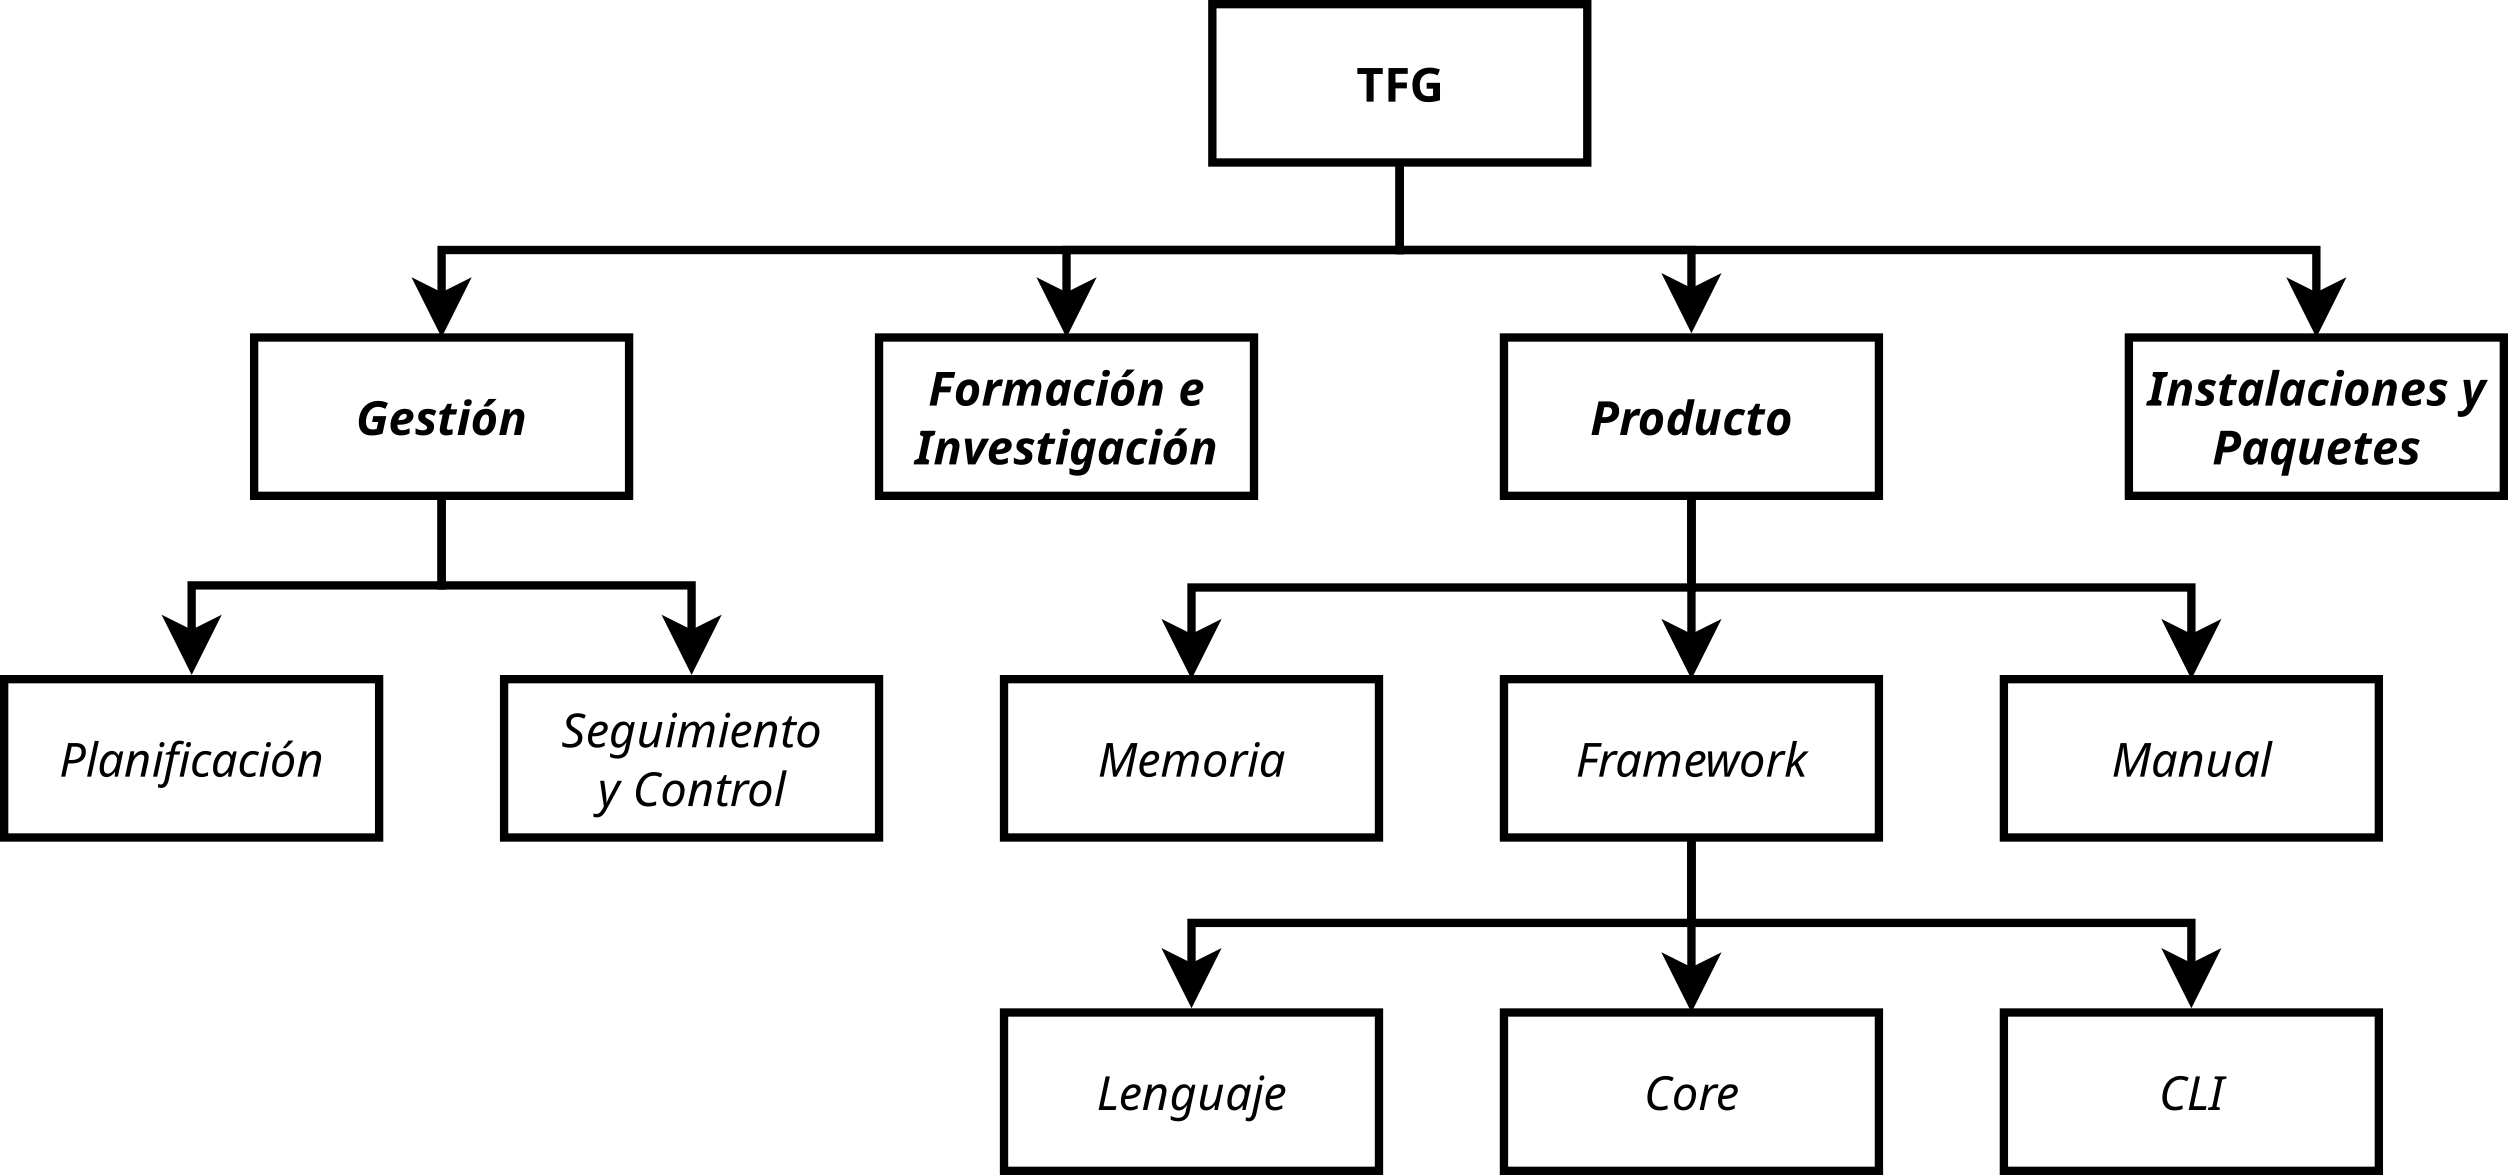
\includegraphics[width=\textwidth]{8-Apéndices/EDT.png}
    \caption{Esquema de Descomposición de Trabajo del Proyecto}
    \label{fig:EDT}
\end{figure}

\cleardoublepage
}

\end{document}